% ==============================================================
%  FCFS Simulation Brief: Main Findings and Discussion Questions
%  Supervisor-ready version -- May 2026
% ==============================================================
\documentclass[10pt]{article}

\usepackage[margin=0.8in]{geometry}
\usepackage{amsmath}
\usepackage{booktabs}
\usepackage{tabularx}
\usepackage{array}
\usepackage{microtype}
\usepackage{parskip}
\usepackage{enumitem}
\usepackage{graphicx}
\usepackage{tcolorbox}
\usepackage{titlesec}
\usepackage[hidelinks]{hyperref}

% Allow compilation from either the repository root or this reports directory.
\graphicspath{{reports/figures/}{figures/}}

% ---- List spacing ----
\setlist[itemize]{leftmargin=1.3em, itemsep=1pt, topsep=2pt, parsep=0pt}
\setlist[enumerate]{leftmargin=1.5em, itemsep=2pt, topsep=2pt, parsep=0pt}

% ---- Column types ----
\newcolumntype{Y}{>{\raggedright\arraybackslash}X}
\newcolumntype{L}[1]{>{\raggedright\arraybackslash}p{#1}}

% ---- Section heading spacing ----
\titleformat{\section}{\normalfont\bfseries\large}{}{0em}{}
\titlespacing*{\section}{0pt}{10pt plus 2pt}{4pt}

\titleformat{\subsection}{\normalfont\bfseries\normalsize}{}{0em}{}
\titlespacing*{\subsection}{0pt}{7pt plus 2pt}{2pt}

% ---- Paragraph spacing ----
\setlength{\parskip}{4pt}

\begin{document}

% ---- Title block ----
\begin{center}
  {\large\bfseries FCFS Simulation Brief: Main Findings and Discussion Questions}\\[3pt]
  Alexandre Sepulveda de Dietrich\quad|\quad
  Supervised by Prof.\ Carri Chan\\[2pt]
  {\small May 2026}
\end{center}
\vspace{2pt}
\noindent\rule{\textwidth}{0.5pt}
\vspace{2pt}

% ============================
%  EXECUTIVE SUMMARY
% ============================
\section*{Executive Summary}

\begin{tcolorbox}[
  colback=gray!7,
  colframe=gray!45,
  boxrule=0.45pt,
  arc=2pt,
  left=8pt, right=8pt, top=6pt, bottom=6pt,
  parbox=true,
]
\textbf{Under this FCFS stress-test baseline, utilization should not be used as
the access summary; report served rate, offered wait, and no-offer share
together.}
Across the 30-seed baseline diagnostic (\(\lambda=100\) arrivals/day,
\(S=32\) slots/day), average utilization is 0.842 while only 0.269 of arriving
patients complete a visit. These metrics have different denominators and respond
to different interventions. Utilization alone understates the access shortfall
at high demand.

\vspace{4pt}
\begin{itemize}
  \item \textbf{Utilization and access decouple by construction.}
    With \(S=32\) slots and \(\lambda=100\) arrivals, the served rate is
    mechanically bounded near \(32/100=0.32\) before behavioral losses.
    Slot fill can be high while most patients are turned away.
  \item \textbf{Baseline losses are post-offer, not no-offer.}
    26.9\% of arrivals are served; 35.5\% balk, 32.5\% cancel, 5.1\%
    no-show, and 0.0\% receive no offer. The horizon does not saturate
    at baseline. Slots are offered, then rejected, canceled, or missed.
  \item \textbf{Suppressing balking does not recover capacity.}
    Removing balking shifts utilization by \(-0.001\) and served rate by
    \(-0.001\). Losses relabel from balking to no-offer and cancellation.
    The completed-visit count is unchanged.
\end{itemize}

\vspace{3pt}
\textit{Caveat: This is a stress-test model, not a calibrated clinic estimate.
The \(3.1:1\) demand-to-capacity ratio is intentionally severe.}
\end{tcolorbox}

\vspace{5pt}
\noindent\textbf{Discussion questions for next meeting:}
\begin{enumerate}
  \item Should the baseline be recalibrated toward a plausible clinic setting,
    or does the stress-test regime remain useful for probing mechanism?
  \item Should no-offer be reported as a distinct access failure in every
    summary table?
  \item Should no-show probability depend on original offered delay, as
    currently implemented, or on remaining wait closer to the service date?
\end{enumerate}

% ============================
%  KEY EVIDENCE
% ============================
\section*{Key Evidence}

\begin{figure}[h!]
  \centering
  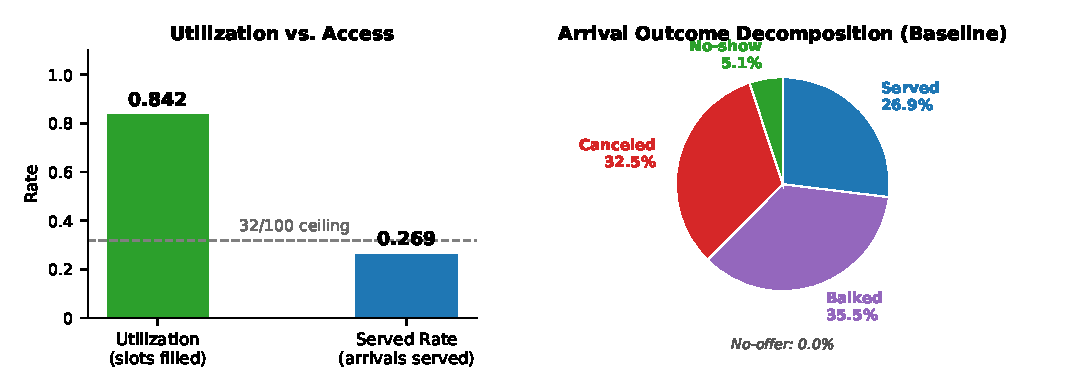
\includegraphics[width=\textwidth]{exec_summary_panel.pdf}
  \caption{Left: utilization vs.\ served rate at baseline. The dashed line marks
    the mechanical ceiling \(32/100=0.32\).
    Right: arrival outcome decomposition over 30 seeds
    (\(\lambda=100\), \(S=32\)).}
  \label{fig:exec}
\end{figure}

\begin{table}[h!]
\centering
\small
\renewcommand{\arraystretch}{1.10}
\begin{tabularx}{0.90\textwidth}{Yrr}
\toprule
Metric & Value & Notes \\
\midrule
Average utilization  & 0.842 & Completed visits per available slot \\
Overall served rate  & 0.269 & Completed visits per arrival \\
Mean offered wait    & 9.29\,d & Delay among patients offered a slot \\
Mean accepted wait   & 8.33\,d & Delay among patients who accepted \\
Overall balking rate & 0.355 & Offered patients who rejected the delay \\
\bottomrule
\end{tabularx}
\caption{Baseline FCFS metrics (30 seeds).}
\label{tab:baseline}
\end{table}

\begin{table}[h!]
\centering
\small
\renewcommand{\arraystretch}{1.10}
\begin{tabularx}{\textwidth}{Yrrr}
\toprule
Metric & Baseline & No-balking & Change \\
\midrule
Average utilization & 0.842 & 0.840 & \(-0.001\) \\
Overall served rate & 0.269 & 0.268 & \(-0.001\) \\
Booked rate         & 0.645 & 0.703 & \(+0.058\) \\
Balked share        & 0.355 & 0.000 & \(-0.355\) \\
Canceled share      & 0.325 & 0.384 & \(+0.059\) \\
No-offer share      & 0.000 & 0.297 & \(+0.297\) \\
Mean accepted wait  & 8.33\,d & 9.45\,d & \(+1.12\,\)d \\
\bottomrule
\end{tabularx}
\caption{No-balking diagnostic, 30 matched seeds.
  Utilization and served rate are essentially unchanged; losses relabel.}
\label{tab:nobalking}
\end{table}

% ============================
%  MAIN TAKEAWAYS
% ============================
\section*{Main Takeaways}

\subsection*{Utilization Is Not Access}

Utilization measures completed visits per available slot; served rate measures
completed visits per arrival. At \(\lambda=100\) and \(S=32\), the served-rate
ceiling is \(32/100=0.32\) before any behavioral losses. The two metrics can
move independently: a policy that fills more slots does not necessarily serve
more patients, and vice versa. Using utilization as a proxy for access will
be misleading whenever the demand-to-capacity ratio is far from one.

\subsection*{Baseline Losses Are Balking and Cancellation}

Every arrival maps to exactly one outcome. At baseline, no-offer is zero: the
system finds a future slot for every arriving patient. Access failures occur
after offers are made, not because the booking horizon is already unavailable
at baseline. Balking (35.5\%) reflects high offered delay; cancellation
(32.5\%) reflects long exposure before service combined with a daily
cancellation probability. The capacity pressure is severe, but the baseline
loss channel is post-offer dropout, not slot unavailability.

\subsection*{Suppressing Balking Does Not Recover Capacity}

Table~\ref{tab:nobalking} is the cleanest diagnostic. Removing balking
raises the booked rate by 0.058 but leaves utilization and served rate
essentially unchanged. The additional bookings extend far into the horizon,
accumulate cancellation exposure, and generate no-offer arrivals once the
horizon fills. Suppressing balking does not recover capacity. It relabels
losses.

\subsection*{Report Offered Wait with No-Offer Share}

Accepted wait is a selective metric: patients who balk at long delays are
excluded. As congestion rises, accepted wait can decrease simply because
high-delay patients opt out, even as access worsens. Offered wait is a better
congestion measure because it is recorded before the balking decision.
However, offered wait excludes no-offer patients. At baseline, no-offer is
zero; but when balking is suppressed, no-offer rises to 0.297 and offered
wait becomes selective in a different way. Report offered wait and no-offer
share together.

\subsection*{Realistic Scenario Check}

A comparison run under a plausible two-class parameterization (\(\lambda=24\),
\(S=20\), demand/supply \(1.2:1\), asymmetric behavioral parameters; 30 seeds) shows what changes when capacity pressure is
reduced. Aggregate outcomes improve substantially: utilization 0.934, served
rate 0.789, balked share 3.3\%, canceled share 12.3\%, no-offer share 0.0\%.
The critical new result is a class-level served-rate gap of 0.220 (Class~1:
0.881, Class~2: 0.661) that is invisible in the aggregate figure. Under pooled
FCFS, asymmetric behavioral parameters create this gap through shared capacity,
not explicit class priority. The reporting recommendation is unchanged: aggregate
metrics alone are insufficient; class-level served rates must also be reported.

% ============================
%  DRIVER HIERARCHY
% ============================
\section*{Driver Hierarchy}

Sensitivity slices and regression screen give a consistent hierarchy;
all coefficients are standardized OLS with HC3 errors.

\begin{itemize}
  \item \textbf{Served rate and offered wait:} driven by arrival rate
    (\(\hat{\beta}=-0.774\) and \(+0.576\); \(p<0.001\)).
    Demand pressure dominates when capacity is fixed.
  \item \textbf{Utilization:} driven by no-show behavior
    (\(\hat{\beta}=+0.512\) threshold, \(-0.423\) step; \(p<0.001\)).
    No-show slots are not rebooked.
  \item \textbf{Balking effect on utilization:} near zero
    (\(\hat{\beta}=+0.016\), \(p=0.72\)). Balking reallocates loss
    channels, not aggregate slot completion.
  \item \textbf{Class access gap:} requires asymmetric parameters.
    Symmetric baseline yields a gap of 0.001; the realistic scenario
    yields 0.220 (see above).
\end{itemize}

% ============================
%  DISCUSSION -- BRIEF EXPANSION
% ============================
\section*{Open Questions}

\begin{enumerate}
  \item \textbf{Recalibrate or keep stress test?}
    The realistic scenario (\(\lambda/S=1.2\)) provides a first check:
    aggregate outcomes improve and the loss-channel mix shifts. The
    stress-test baseline remains useful for mechanism diagnosis. The open
    question is which parameter regime should serve as the main reference
    case, and what clinical inputs justify that choice.

  \item \textbf{Report no-offer as distinct access failure?}
    Zero at baseline, but appears immediately under higher \(\lambda\) or
    without balking. Including it in every summary table prevents silent
    omissions when parameter regimes change.

  \item \textbf{No-show rule: original delay or residual wait?}
    The current rule uses original booking delay, not residual wait.
    Switching to residual wait would make offered delay a more direct
    driver of utilization and would likely alter the regression hierarchy.
\end{enumerate}

% ============================
%  WHERE TO DIG
% ============================
\section*{Where to Dig}

This brief stands alone. The table below points to the full note
(\texttt{fcfs\_metric\_analysis\_note.pdf}) for details.

\vspace{2pt}
\begin{tabularx}{\textwidth}{L{0.38\textwidth}Y}
\toprule
Topic & Full-note reference \\
\midrule
Baseline setup and metric definitions & Sections 2.1--2.3 \\
Utilization vs.\ served-rate gap & Section 2.3; Section 5 \\
Outcome decomposition detail & Section 3.1, Table~2 \\
No-balking diagnostic & Section 3.2, Table~3 \\
Sensitivity driver hierarchy & Sections 6.1--6.5 \\
Regression coefficients (full table) & Appendix~D \\
Class gap and equity & Sections 6.5, 8 \\
Discussion and caveats & Sections 9--10 \\
Realistic scenario comparison & \texttt{realistic\_baseline\_comparison.pdf} \\
\bottomrule
\end{tabularx}

\end{document}
